%%
%% $Id$
%%
%% Copyright (c) 2007-2008 Christian Fehler
%% Copyright (c) 2007-2008 Benjamin Mies
%%


\chapter{Automaten}\label{Machines}


\section{Graphenansicht}


\subsection{Automatendarstellung mit JGraph}

TODOBM


\subsection{Anpassung von JGraph}

TODOCF


\section{Tabellen}


\subsection{Übergangstabelle}

Während der Entwicklung und ersten Tests des \gtitools kam der Wunsch auf,
einen Automaten nicht nur graphisch zu bearbeiten, sondern auch in der
Übergangstabelle. Dadurch soll es dem Benutzer ermöglicht werden, Übergänge
schneller anzulegen, als es bei der normaler Methode in der Graphenansicht der
Fall wäre. Um diese neue Methode zu implementieren wurden einige verschiedene
Umsetzungen diskutiert. Zur Diskusion standen unter anderen, dass in jeder
Zelle der Tabelle ausgewählt werden kann, zu welchen Zuständen ein Übergang
existiert. Diese Auswahl hätte allerdings bei der Umsetzung schlecht
ausgesehen, zumindest bei hinreichend vielen Zuständen. Aus diesem Grund wurde
dieser Ansatz verworfen.\vspace{10pt}

\begin{figure}[h!]
\begin{center}
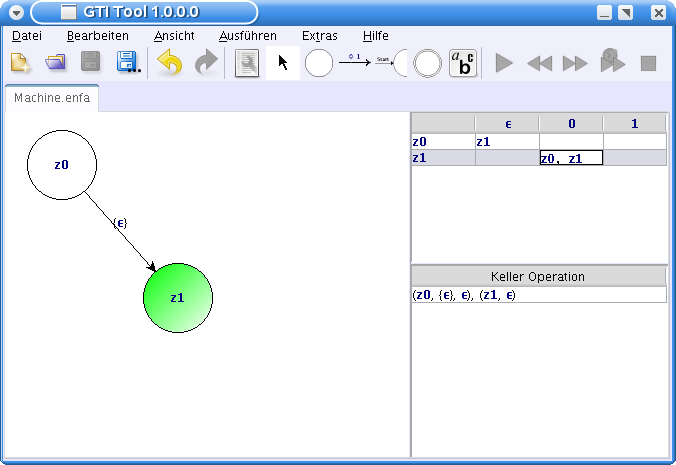
\includegraphics[width=12cm]{../images/machine_table.png}
\caption{Übergangstabelle}
\end{center}
\end{figure}

Als nächste mögliche Umsetzung wurde diskutiert, ob es technisch möglich sei,
in jede Zelle einen Parser zu verwenden. Dieser Parser musste so implementiert
werden, dass er einen oder mehrere, durch Komma getrennte Zustände als Eingabe
akzeptiert. Im Kapitel \ref{Parser} werden einige kontextsensitive Bedingungen
angesprochen, die auch bei dem hier vorliegenden Parser verwendet werden
mussten, da es dem Benutzer nicht möglich sein sollte, einen oder mehrere
Zustände anzugeben, die nicht im Graphen vorkommen. Der Parser als solches
konnte leicht implementiert werden, es gab allerdings einige technische
Probleme diesen in jede Zelle zu implementieren. Diese Probleme konnten gelöst
werden, so dass der Benutzer nun in der Lage ist, Übergänge per Tabelle
anzulegen, zu modifizieren und zu löschen.


\subsection{Keller Operationen Tabelle}

TODOBM


\section{Wort-Navigation}


\subsection{Deterministische Navigation}

TODOBM


\subsection{Navigation im Kellerautomaten mit Auswahl}

TODOCF


\subsection{Zustands Pfad}

Bei Verwendung eines nicht deterministischen Automaten stellte sich bei der
Wort Navigation die Frage, auf welchem Pfad die aktuell aktiven Zustände
erreicht wurden. Es wurden verschiedene Umsetzungen in Betracht gezogen, dem
Benutzer die Ausgabe darzustellen. Es wurde schließlich entschieden, die
Zustände auf dem Weg zu den aktuell aktiven Zuständen darzustellen. Zwischen
diesen Zuständen werden die verwendeten Übergänge, sowie die verwendeten
Symbole an den Übergängen dargestellt, bzw. hervorgehoben. Da unter Umständen
viele Zustands Pfade vorhanden sein können, werden diese anhand der Anzahl der
verwendeten Zustände sortiert, somit werden die kürzesten Pfade zuerst
angezeigt.\vspace{10pt}

\begin{figure}[h!]
\begin{center}
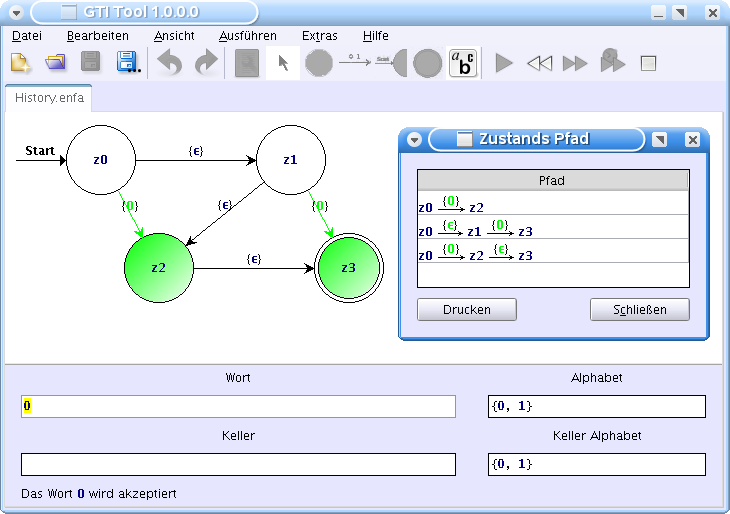
\includegraphics[width=12cm]{../images/history_path.png}
\caption{Zustands Pfad}
\end{center}
\end{figure}

Der implementierte Algorithmus geht rückwärts vor, startet also bei den aktuell
aktiven Zuständen und geht alle Pfade zurück, bis alle, bis jetzt gelesenen
Symbole abgearbeitet sind. Startet der berechnete Pfad dann in dem
Startzustand, wurde ein gültiger Pfad erkannt. Bei der Implementierung des
Algorithmus musste eine Zykluserkennung umgesetzt werden, da es sonst möglich
war in eine Endlosschleife zu geraten, welche durch $\epsilon$-Übergänge
verursacht wurde.


\section{Erreichbare Zustände}\label{ReachableStates}

Nach dem in \ref{ConverToMachine} nachzulesenen Umwandeln eines nicht
deterministischen in einen deterministischen Automaten unter Verwendung der
Potenzautomatenkonstruktion stellte sich die Frage, wie die nicht erreichbaren
Zustände erkannt und entfernt werden können. Dieses Problem betrifft aber nicht
nur umgewandelte Automaten, sondern ganz allgemein, jeden erstellten
Automaten.\vspace{10pt}

Bei der Umsetzung sollte im Vordergrund stehen, dass der Benutzer mit sehr
kleinen Schritten verdeutlicht bekommt, wie der zugrunde liegende Algorithmus
arbeitet, so dass diese Arbeitsweise sehr einfach nachzuvollziehen
ist.\vspace{10pt}

\begin{figure}[h!]
\begin{center}
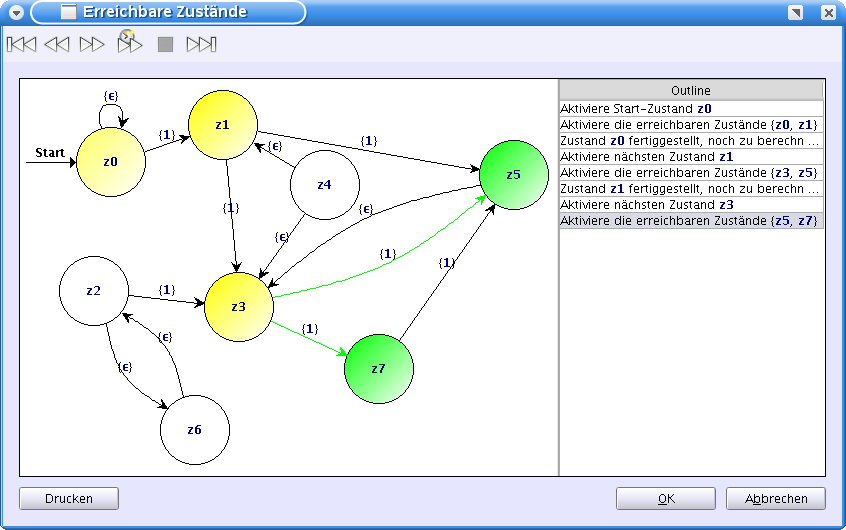
\includegraphics[width=12cm]{../images/reachable_states.png}
\caption{Erreichbare Zustände}
\end{center}
\end{figure}

Der verwendete Algorithmus besteht aus drei Phasen. In der ersten Phase wird ein
noch nicht abgearbeiteter Zustand ausgewählt, zu Beginn wird mit dem Startzustand
begonnen. In der zweiten Phase werden die von diesem Zustand aus direkt
erreichbaren Zustände berechnet und dem Benutzer hervorgehoben dargestellt. In
der dritten Phase werden alle bis jetzt zu erreichenden Zustände hervorgehoben.
Gleichzeitig bekommt der Benutzer in der Outline mitgeteilt, welcher Zustand
jetzt fertiggestellt ist und welche noch berechnet werden müssen. Durch diese
sehr feine Unterteilung, soll ein besseres Verständnis des Algorithmus erreicht
werden.
